L’objectif de la présente étude est de simuler l’aéroport de Brest afin de dimensionner de façon optimale ses futures évolutions. 

Pour cela nous avons réalisé une simulation à événement discret, dans laquelle nous avons étudié l'état de l'aéroport à chaque événement.

L'aéroport possède un seul terminal avec 4, 6 ou 8 emplacements; une seule piste (6L/24R) et deux taxiways entre l'aérogare et la piste, un pour l'atterrissage et l'autre pour le décollage. Cette configuration est représentée sur la figure \ref{aeroport}.

\begin{figure}[h]
	\centering
 	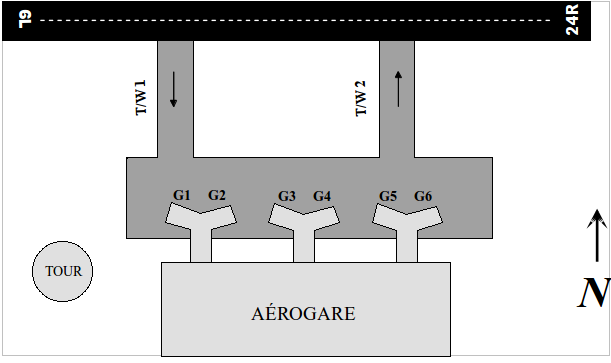
\includegraphics[scale=0.32]{aeroport.png}
	\caption{\label{aeroport} Boucle de simulation}
\end{figure}

La simulation porte une attention particulière sur les arrivées des avions et les temps qu'ils mettent à effectuer les différentes étapes, de leur arrivée dans l'espace aérien de l'aéroport jusqu'à leur départ.
La simulation a pour objectifs de déterminer les surcharges éventuelles de l’aéroport et leur contexte, en fonction des infrastructures disponibles.
Elle est donc modulable, afin de faire varier ces infrastructures, notamment en modifiant les nombres de portes d’accès et de pistes, et d’étudier les conséquences de ces variations.


Le livrable final est composé du programme de simulation (sous la forme d'un projet JAVA compilable) et d'une étude des données générées par ce programme. Cette étude déterminera notamment les moyennes de fréquentation journalière, de retards, de temps d'attentes avant atterrissage.
